\documentclass{beamer}
\beamertemplatenavigationsymbolsempty
\usefonttheme[stillsansseriflarge]{serif}
\setbeamertemplate{footline}[frame number]
\usepackage[type1]{libertine}
\usepackage{bbold}
\usepackage{tikz}
%\usetheme{Warsaw}
% \usetheme{Goettingen} alternative themes
% \usetheme{Hannover}
% \usetheme{Marburg}
% \usetheme{PaloAlto}
%\title[Geek’s Night : Velha-A-Branca – March 2, 2010]{Introduction of Aspect Oriented Programming}
\author{Shih-Kai Lin}
%\institute[UM]{University of Minho}
\date{}
\title{\texorpdfstring{$\nu_\mu e$}{nu-e} kinematics \& dynamics}
\begin{document}
\begin{frame}
\titlepage
\end{frame}
\begin{frame}[allowframebreaks]{}

\begin{figure}
\centering
  \begin{tikzpicture}
    \draw [>=latex, <->] (-1,0) node [right] {$z$} -- (-1.5,0) -- (-1.5,.5) node [above] {$x$};
    \draw [>=latex, ->, very thick, red] (.9,1) node [left] {$(E_\nu,\vec{p}_\nu)$} -- (2.9,1);
    \draw [dashed] (3,1) -- +(3,0);
    \draw [>=latex, ->, very thick, red] (3,1) -- +(1.5,1.5) node [above right] {$(E',\vec{p}'_\nu)$};
    \draw (3.3,1) arc (0:45:0.3) node [right] {$\phi$};
    \draw [>=latex, ->, very thick, cyan] (3,1) -- +(2.598,-1.5) node [below right] {$(E_e,\vec{p})$};
    \draw (3.6,1) arc (0:-30:.6) node [right] {$\theta$};
  \end{tikzpicture}
\end{figure}


A neutrino collides with an electron at rest. Write down the 4-momenta of the neutrino and the electron in the lab frame. Suppose the neutrino is massless. Before collision we have ($\hbar=c=1$)

\framebreak

\begin{eqnarray}
\mathbb{p}_\nu &=&(E_\nu,0,0,E_\nu) \label{eq:pnu}\\
\mathbb{p}_e&=&(m,0,0,0) \label{eq:pe}
\end{eqnarray}
, where $m$ is the electron rest mass, and $E_\nu$ is the total energy of the incident neutrino.
After collision, we have
\begin{eqnarray}
\mathbb{p'}_\nu &=&(E',E'\sin\phi,0,E'\cos\phi) \label{eq:ppnu} \\
\mathbb{p'}_e &=& (E_e,-p\sin\theta,0,p\cos\theta) \label{eq:ppe}
\end{eqnarray}


The total 4-momentum before collision is
\begin{equation} \label{eq:ptot}
  \mathbb{P} = (E_\nu+m,0,0,E_\nu)
\end{equation}
The total 4-momentum after collision is
\begin{equation} \label{eq:pptot}
  \mathbb{P}' = (E'+E_e,-p\sin\theta+E'\sin\phi,0,p\cos\theta+E'\cos\phi)
\end{equation}

\framebreak

Since total 4-momentum is conserved before and after collision, we have equations
\begin{eqnarray}
  E'+E_e &=& E_\nu+m \label{eq:E} \\
  -p\sin\theta+E'\sin\phi &=& 0 \label{eq:ptotx} \\
  p\cos\theta+E'\cos\phi &=& E_\nu \label{eq:ptotz}
\end{eqnarray}

Rearranging equations~\eqref{eq:ptotx} and~\eqref{eq:ptotz}, squaring, and adding them, we eliminate $\phi$ and obtain

\begin{equation}
  E'^2 = E^2_\nu -2E_\nu p\cos\theta+p^2
\end{equation}
If we eliminate $E'$ with Eq.~\eqref{eq:E}, and employ the energy-momentum relation $E_e^2=p^2+m^2$ once, we obtain
\begin{equation} \label{eq:lasteq}
  p\cos\theta=(E_e-m)\left( 1+\frac{m}{E_\nu} \right)
\end{equation}

\framebreak

By squaring Eq.~\eqref{eq:lasteq}, and employing the energy-momentum relation again, we arrive at the answer
\begin{equation} \label{eq:Ee}
  \boxed{\frac{E_e}{m}=\frac{\left( 1+\frac{m}{E_\nu} \right)^2+\cos^2\theta}{\left( 1+\frac{m}{E_\nu} \right)^2-\cos^2\theta}}
\end{equation}

If we choose to eliminate $\theta$ and $E_e$, we get
\begin{equation} \label{eq:Ep}
  E'=\frac{E_\nu m}{E_\nu(1-\cos\phi)+m}
\end{equation}

\framebreak

Rearranging and dividing Eq.~\eqref{eq:ptotx} by Eq.~\eqref{eq:ptotz}, we have
\begin{equation}
  \cot\theta=\frac{\frac{E_\nu}{E'}-\cos\phi}{\sin\phi}=\left( 1+\frac{E_\nu}{m} \right)\tan\left( \frac{\phi}{2} \right)
\end{equation}
, where we have used Eq.~\eqref{eq:Ep} for $E_\nu/E'$.

For a neutrino scattering angle $0\leq\phi\leq\pi$, the range of the electron scattering angle is
\begin{equation}
  \boxed{0\leq\theta\leq\frac{\pi}{2}}
\end{equation}
\end{frame}

\begin{frame}[allowframebreaks]{kinematical cut}
  For small $\theta$, Eq.~\eqref{eq:Ee} becomes $E_e\theta^2/2m\approx 1$. However, since we have the \emph{exact} formula for $E_e$, we can actually plot the function
\begin{equation} \label{eq:exact_cut_function}
  f(\theta)=\frac{E_e\theta^2}{2m}=\frac{\left( 1+\frac{m}{E_\nu} \right)^2+\cos^2\theta}{\left( 1+\frac{m}{E_\nu} \right)^2-\cos^2\theta}\cdot\frac{\theta^2}{2}
\end{equation}
and see how close it is to $1$.

\framebreak
\begin{figure}
\centering
  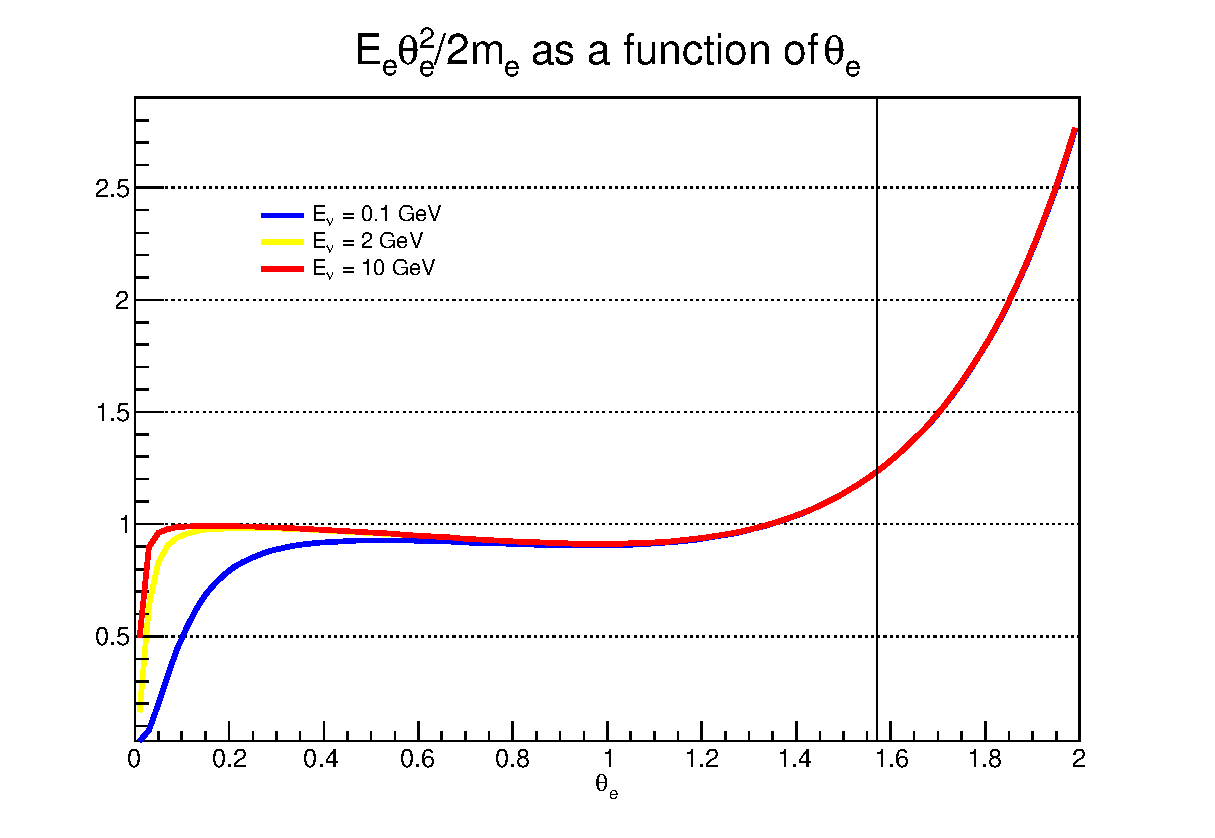
\includegraphics[width=\textwidth]{figures/cut_func_with_angle.eps}
\end{figure}

\end{frame}

\begin{frame}{$\nu_\mu e$ dynamics I}
\tiny
The differential cross section of $\nu_\mu e$ scattering is\footnotemark
\begin{equation}
  \begin{aligned}
  \frac{d\sigma}{d\cos\theta} & = \sigma_0 \frac{4E_\nu^2(m_e+E_\nu)^2\cos\theta}{\left[ (m_e+E_\nu)^2-E_\nu^2\cos^2\theta \right]^2} \\
  & \times \left[ g_1^2 + g_2^2\left( 1-\frac{2m_eE_\nu\cos^2\theta}{(m_e+E_\nu)^2-E_\nu^2\cos^2\theta} \right)^2 -g_1g_2
  \frac{2m_e^2\cos^2\theta}{(m_e+E_\nu)^2-E^2_\nu\cos^2\theta} \right]
  \end{aligned}
\end{equation}
, where
\begin{eqnarray*}
  \sigma_0 &=& \frac{2G_F^2m_e^2}{\pi}\approx 88.06\times 10^{-46} \text{ cm}^2 \\
  g_1 &=& -\frac{1}{2}+\sin^2\theta_W \approx -0.27 \\
  g_2 &=& \sin^2\theta_W \approx 0.23
\end{eqnarray*}
\footnotetext[1]{\tiny Giunti C. and Kim C. W., \textit{Fundamentals of Neutrino Physics and Astrophysics}, 2007}
\end{frame}

\begin{frame}{$\nu_\mu e$ dynamics II}
\begin{figure}
\centering
  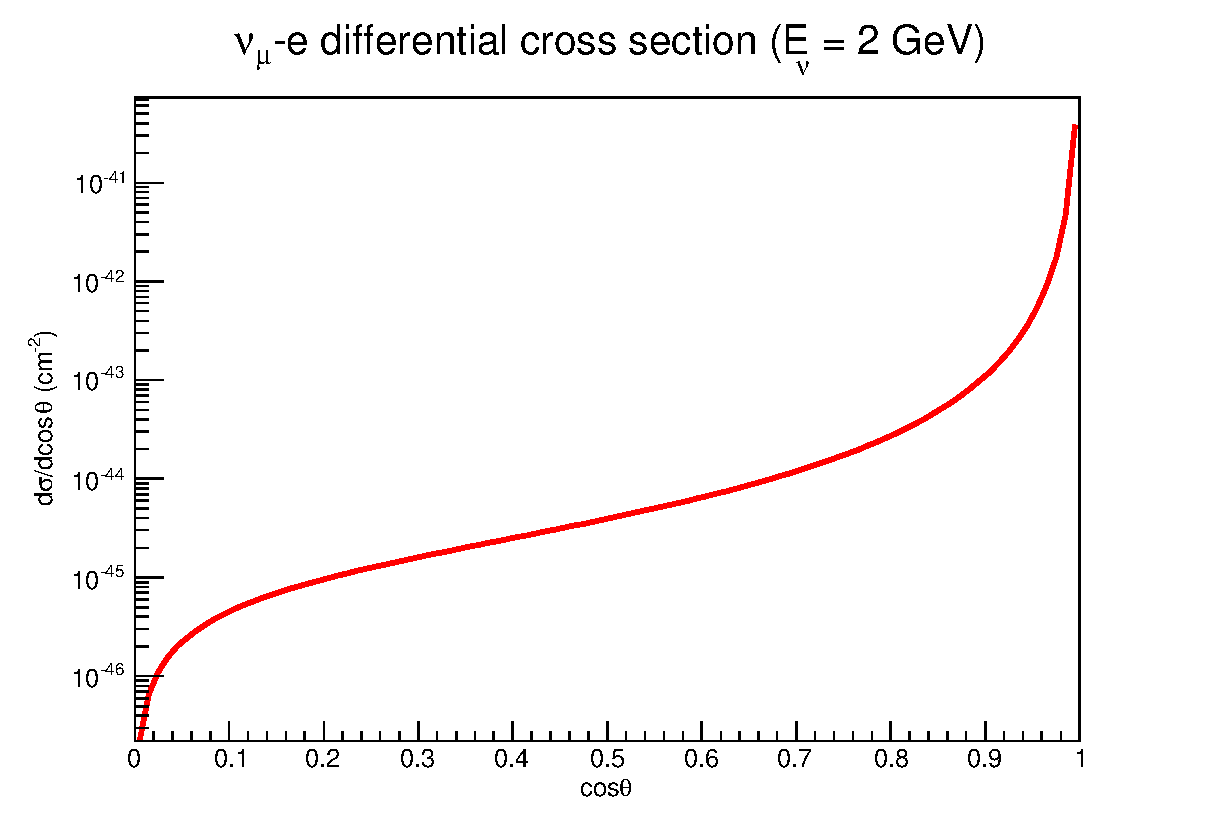
\includegraphics[width=\textwidth]{figures/diff_xsec.eps}
\end{figure}
\end{frame}

\end{document}